\documentclass[conference]{IEEEtran}

\usepackage{graphicx}
\usepackage{tikz}
\usepackage{pgfplots}
\pgfplotsset{compat=1.18}
\usetikzlibrary{arrows.meta,positioning}

\begin{document}

% ================= Title =================
\begin{center}
    {\LARGE \textbf{Figures and Tables for}\\[0.5em]
    \Large ``FeFET CMOS 0.18~$\mu$m Integration Study''}
\end{center}
\vspace{1em}

% ================= Page 1 =================
\section*{Figures and Tables (Process Integration)}

% -------- Fig.1 --------
\begin{figure}[!t]
\centering
% TikZ 図をここに
\caption{Placement of the FeFET gate-last module within the 0.18~$\mu$m CMOS baseline (vertical layout).}
\end{figure}

\vspace{2em} % Fig.1 と Table I の間隔を確保

% -------- Table I --------
\begin{table}[!t]
\centering
\caption{Added masks / process steps relative to baseline logic.}
\begin{tabular}{|c|c|l|}\hline
Step & Mask & Comment\\ \hline
FE metal gate & +1 & Reuse analog option route\\
FE anneal & 0 & Performed in BEOL furnace (no extra mask)\\ \hline
\end{tabular}
\end{table}

\newpage

% ================= Page 2 =================
\section*{Figures and Tables (Reliability Data)}

% -------- Fig.2 --------
\begin{figure}[!t]
\centering
% Endurance グラフ
\caption{Schematic endurance behavior of HZO-FeFETs in a 0.18~$\mu$m flow.}
\end{figure}

% -------- Fig.3 --------
\begin{figure}[!t]
\centering
% Wake-up と Retention 縦並び
\caption{Wake-up (top) and retention projection at 85$^\circ$C (bottom).}
\end{figure}

% -------- Fig.4 --------
\begin{figure}[!t]
\centering
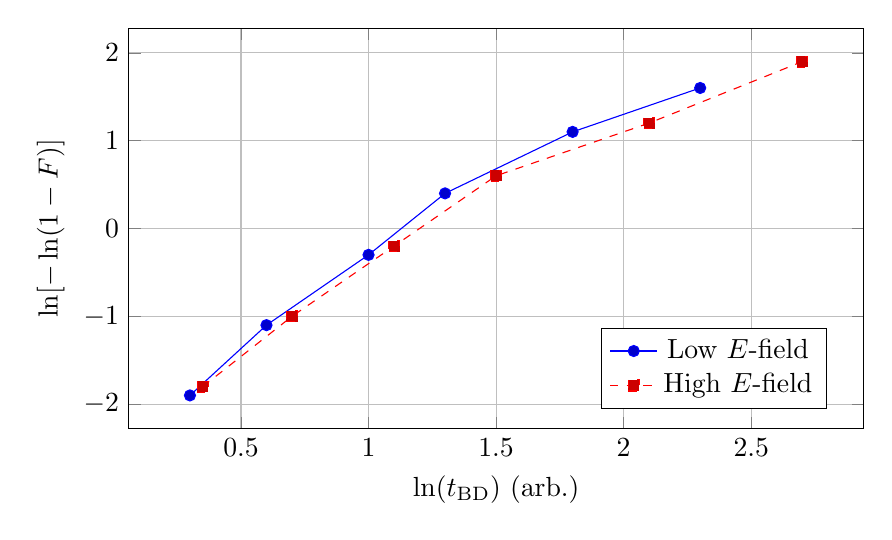
\begin{tikzpicture}
\begin{axis}[
  width=0.9\linewidth,height=0.55\linewidth,
  xlabel={$\ln(t_{\mathrm{BD}})$ (arb.)},
  ylabel={$\ln[-\ln(1-F)]$}, grid=both,
  legend style={at={(0.95,0.05)},anchor=south east} % 凡例を右下へ
]
\addplot+[mark=*] coordinates {(0.3,-1.9) (0.6,-1.1) (1.0,-0.3) (1.3,0.4) (1.8,1.1) (2.3,1.6)};
\addlegendentry{Low $E$-field}
\addplot+[mark=square*, dashed] coordinates {(0.35,-1.8) (0.7,-1.0) (1.1,-0.2) (1.5,0.6) (2.1,1.2) (2.7,1.9)};
\addlegendentry{High $E$-field}
\end{axis}
\end{tikzpicture}
\caption{TDDB Weibull representation at two stress fields (illustrative).}
\end{figure}

\end{document}
